\documentclass[10pt,english]{article}
\usepackage{geometry}
 \geometry{verbose,tmargin=2cm,bmargin=2cm,footskip=1cm}
\usepackage{babel}
\usepackage{bm}
\usepackage{amssymb}
\usepackage{amsmath}
\usepackage{multirow}
\usepackage{graphicx}
\usepackage{setspace}
\onehalfspacing


\def\vss{\vspace{1cm}}
\def\vs{\vspace{0.2cm}}

\begin{document}

\noindent
\centerline{
\textbf{\large Numerical Methods for the Solution of Differential Equations (AM 213B)}}\\
\centerline{{\bf Homework 3 - grading form}}
%
\centerline{\line(1,0){480}}\vspace{.cm}

\vspace{0.2cm}
\flushleft{\bf Name:} Dante Buhl
\vs
\flushleft{\bf Final score:} write your final score here, for instance, 93/100.

\vss\noindent
\centerline{\bf Point allocation explanation}


\vs
{\bf Question 1 (40/40 points):} The code correctly computes the solution using
a Linear Solve function from Lapack. Both plots produced match those shown in
the solution. 

\vs   
{\bf Question 2 (57/60 points):} The analytical solution produced matched that in
the solutions. The only distinction is the differnce in how the $\sin$ term is
written but they are equivalent. The produced plot of the analytical solution
matches. Finite Difference method produces the same solution.
Gauss-Chebyshev-Lobatto method produces the same solution. The error plot for
the Finite Difference Method matches. The plot for the spectral method is very
similar however not exactly the same. Partial credit is given here since the
plot has very similar features and resembles the plot in the solutions except
for the bump back to $10^{-6}$. 

\vs
{\bf Extra Credit Question (30/30 points):} I would like to petition for more
points in this section. What I submitted did not produce the correct solution so
there was no use in submitting anything at the time. Howver, going back through
the code, I noticed that there was an error in the $\Delta t$ value I passed to the
routine. It was 10 times larger than it was supposed to be and this caused the
AB2 method to become unstable and blow up. After I fixed this issue, I tested
the code and obtained the correct result. I have attached the plots that my code
now produces here, so that they may be considered. I believe I deserve full
credit for this portion of the assignment, but if you do not agree I will be
happy with the 10 points of partial credit for having a numerical algorithm but
it not working properly. 

\begin{figure}[ht]
    \centering
    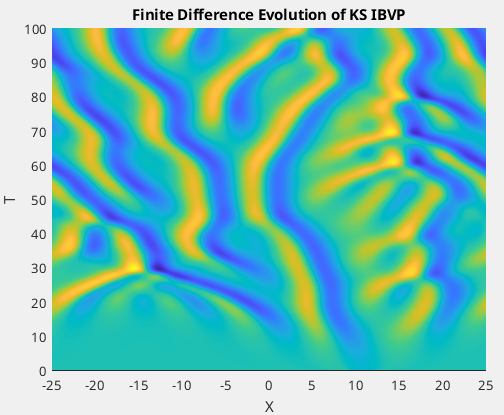
\includegraphics[width=.5\textwidth]{q3_colormap.png}
    \caption{2D Colormap of Numerical Solution to (3)}
\end{figure}
\begin{figure}[ht]
    \centering
    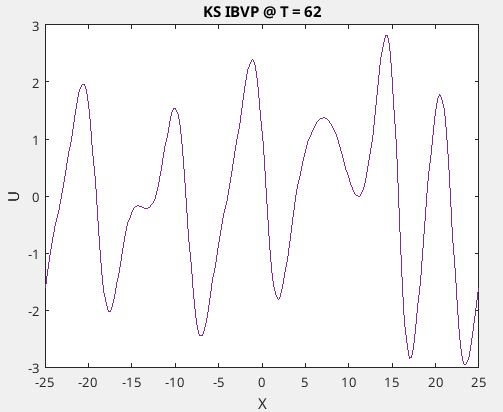
\includegraphics[width=.5\textwidth]{q3t62.png}
    \caption{Cross Section of Numerical Solution to (3) at T = 62}
\end{figure}

\end{document}
